\documentclass[12pt]{article}

\usepackage{ishn}

\makeindex[intoc]

\begin{document}

\hypersetup{pageanchor=false}
\begin{titlepage}
	\begin{center}
		\vspace*{1em}
		\Huge
		\textbf{III General Relativity}

		\vspace{1em}
		\large
		Ishan Nath, Michaelmas 2024

		\vspace{1.5em}

		\Large

		Based on Lectures by Prof. Claude Warnick

		\vspace{1em}

		\large
		\today
	\end{center}
	
\end{titlepage}
\hypersetup{pageanchor=true}

\tableofcontents

\newpage

% lecture 1

\setcounter{section}{-1}

\section{Introduction}%
\label{sec:intro}

Office hours: 8:40AM MWF, in MR2. Normal room E1.14. Will follow roughly Reall's course.

General relativity is our best theory of gravitation on the largest scales. It is:
\begin{itemize}
	\item Classical : No quantum effects.
	\item Geometrical: Space and time are combined in a curved spacetime.
	\item Dynamical: In contrast to Newton's theory of gravity, Einstein's gravitational field has its own non-trivial dynamics.
\end{itemize}

\newpage

\section{Differentiable Manifolds}%
\label{sec:diff_man}

The basic object of study in differential geometry is the (differentiable) manifold. This is an object which `locally looks like $\mathbb{R}^n$', and has enough structure to let us do calculus.

\begin{definition}
	A \emph{differentiable manifold}\index{differentiable manifold}\index{manifold} of dimension $n$ is a set $M$, together with a collection of coordinate charts $(O_\alpha, \phi_\alpha)$, where:
	\begin{itemize}
		\item $O_\alpha \subseteq M$ are subsets of $M$ such that
			\[
			\bigcup_{\alpha} O_\alpha = M.
			\]
		\item $\phi_\alpha$ is a bijective map from $O_\alpha$ to $U_\alpha$, an open subset of $\mathbb{R}^n$.
		\item If $O_\alpha \cap O_\beta \neq \emptyset$, then
			\[
			\phi_\beta \circ \phi_\alpha^{-1}
			\]
			is a smooth map from $\phi_\alpha(O_\alpha \cap O_\beta) \subseteq U_\alpha$ to $\phi_\beta(O_\alpha \cap O_\beta) \subseteq U_\beta$.
	\end{itemize}
	
\end{definition}

\begin{center}
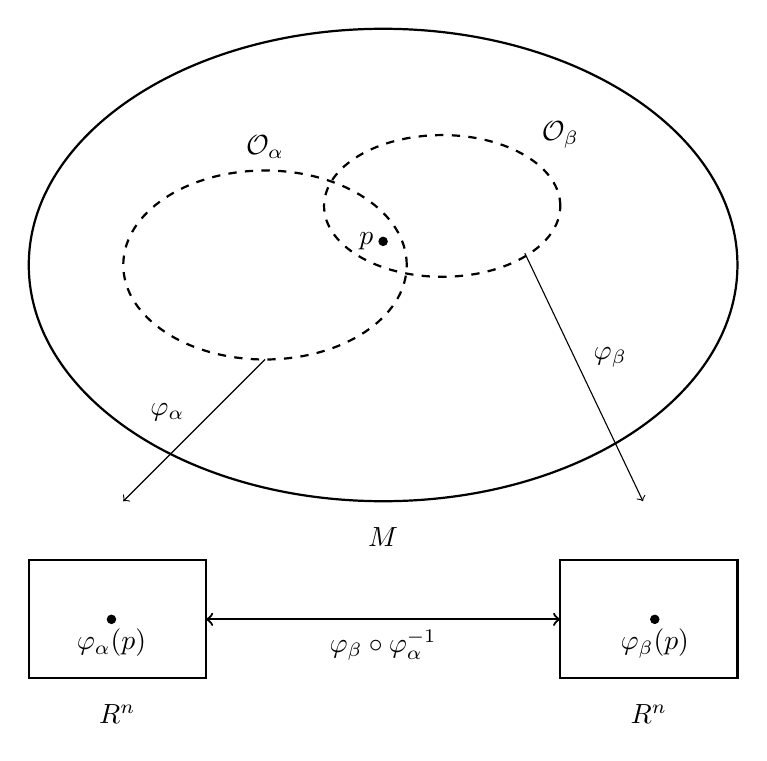
\begin{tikzpicture}[scale=1.5]

    % Define the manifold M
    \draw[thick] (0,0) ellipse (3 and 2);
    \node at (0,-2.3) {$M$}; % Label for M

    % Define open sets O_alpha and O_beta
    \draw[thick, dashed] (-1,0) ellipse (1.2 and 0.8);
    \node at (-1,1) {$\mathcal{O}_\alpha$};
    
    \draw[thick, dashed] (0.5,0.5) ellipse (1 and 0.6);
    \node at (1.5,1.1) {$\mathcal{O}_\beta$};



    % Define arrows to Euclidean spaces
    \draw[->] (-1,-0.8) -- (-2.2,-2) node[midway, above left] {$\varphi_\alpha$};
    \draw[->] (1.2,0.1) -- (2.2,-2) node[midway, above right] {$\varphi_\beta$};

    % Define Euclidean spaces
    \draw[thick] (-3,-2.5) rectangle (-1.5,-3.5);
    \node at (-2.25,-3.8) {$\mathbb{R}^n$};

    \draw[thick] (3,-2.5) rectangle (1.5,-3.5);
    \node at (2.25,-3.8) {$\mathbb{R}^n$};

    % Transition map between charts
    \draw[<->, thick] (-1.5,-3) -- (1.5,-3) node[midway, below] {$\varphi_\beta \circ \varphi_\alpha^{-1}$};

    % Points in the manifold and Euclidean space
    \filldraw (0,0.2) circle (1pt) node[left] {$p$};
    %\filldraw (1.5,0.1) circle (1pt) node[right] {$p$};

    \filldraw (-2.3,-3) circle (1pt) node[below] {$\varphi_\alpha(p)$};
    \filldraw (2.3,-3) circle (1pt) node[below] {$\varphi_\beta(p)$};

\end{tikzpicture}
\end{center}

\begin{remark}
	\begin{itemize}
		\item[]
		\item We could replace smooth with finite differentiability (e.g. $k$-times differentiable).
		\item The charts define a topology on $M$: $U \subseteq M$ is open if and only if $\phi_\alpha(U \cap O_\alpha)$ is open in $\mathbb{R}^n$ for all $\alpha$. Every open subset of $M$ is itself a manifold, by restricting the charts to $U$.
	\end{itemize}
\end{remark}

The collection $\{(O_\alpha, \phi_\alpha)\}$ is called an \emph{atlas}\index{atlas}. Two atlases are \emph{compatible}\index{compatible atlases} if their union is an atlas.

An atlas $A$ is \emph{maximal}\index{maximal atlas} if there exists no atlas $B$ which is compatible with $A$, and strictly larger than $A$. Every atlas is contained in a maximal atlas (by taking the union of all compatible atlases). Hence we can assume without loss of generality that we work with a maximal atlas.

\begin{exbox}
	\begin{enumerate}
		\item If $U \subseteq \mathbb{R}^n$ is open, we can take $O = U$, and $\phi : U \to \mathbb{R}^n$ to be the identity on $U$. Then $\{(O, \phi)\}$ is an atlas.
		\item Take $S^1$. If $p \in S^1 \setminus \{(-1, 0)\} = O_1$, there is a unique $\theta_1 \in (-\pi, \pi)$ such that
			\[
			p = (\cos \theta_1, \sin \theta_1).
			\]
			If $p \in S^1 \setminus \{(1, 0)\} = O_2$, there is a unique $\theta_2 \in (0, 2\pi)$ such that
			\[
			p = (\cos \theta_2, \sin \theta_2).
			\]
			These maps from $(-\pi, \pi)$ and $(0, 2\pi)$ to $O_1, O_2$ give $\phi_1^{-1}, \phi_2^{-1}$ respectively. Note that $\phi_1(O_1 \cap O_2) = (-\pi, 0) \cup (0, \pi)$, and the transition function is
			\[
			\phi_2 \circ \phi_1^{-1} (\theta) = 
			\begin{cases}
				\theta & \theta \in (0, \pi), \\
				\theta + 2 \pi & \theta \in (-\pi, 0).
			\end{cases}
			\]
			This is smooth where defined, and similarly for $\phi_2 \circ \phi_1^{-1}$. Hence $S^1$ is a manifold.
		\item More generally, we can consider $S^n$, and can define charts by stereographic projections. If $\{\mathbf{E}_1, \ldots, \mathbf{E}_{n+1}\}$ is the standard basis for $\mathbb{R}^{n+1}$, and $\{\mathbf{e}_1, \ldots, \mathbf{e}_n\}$ is the standard basis for $\mathbb{R}^n$, write
			\[
			\mathbf{P} = P^1 \mathbf{E}_1 + \cdots + P^{n+1} \mathbf{E}_{n+1}.
			\]
			Set $O_1 = S^n \setminus \{\mathbf{E}_{n+1}\}$, and write
			\[
			\phi_1(\mathbf{P}) = \frac{1}{1 - P^{n+1}}(P^1 \mathbf{e}_1 + \cdots + P^n \mathbf{e}_n).
			\]
			In a similar way we may define $O_2, \phi_2$, for $-\mathbf{E}_{n+1}$. The transition map is then
			\[
			\phi_2 \circ \phi_1^{-1}(\mathbf{x}) = \frac{\mathbf{x}}{|\mathbf{x}|^2},
			\]
			which is smooth on $\mathbb{R}^n \setminus \{0\} = \phi_1 (O_1 \cap O_2)$.
	\end{enumerate}
\end{exbox}

% lecture 2

``Nice'' surfaces in $\mathbb{R}^n$ are manifolds with no cusps, cornered or self-intersections, for example $S^n \subseteq \mathbb{R}^{n+1}$.

\subsection{Smooth Functions on Manifolds}%
\label{sub:smooth_fn}

Suppose $M, N$ are manifolds of dimension $n, n'$ respectively. Let $f : M \to N$.

Then let $p \in M$, and pick charts $(O_\alpha, \phi_\alpha)$ for $M$, and $(O_\beta', \phi_\beta')$ for $N$, with $p \in O_\alpha$ and $f(p) \in O_\beta$. Then,
\[
\phi_\beta' \circ f \circ \phi_\alpha^{-1}
\]
maps a neighbourhood of $\phi_\alpha(p)$ in $U_\alpha \subseteq \mathbb{R}^n$, to $U_\beta' \in \mathbb{R}^{n'}$. If this function is smooth for all possible choices of this chart, we say that $f : M \to N$ is smooth.

\begin{center}
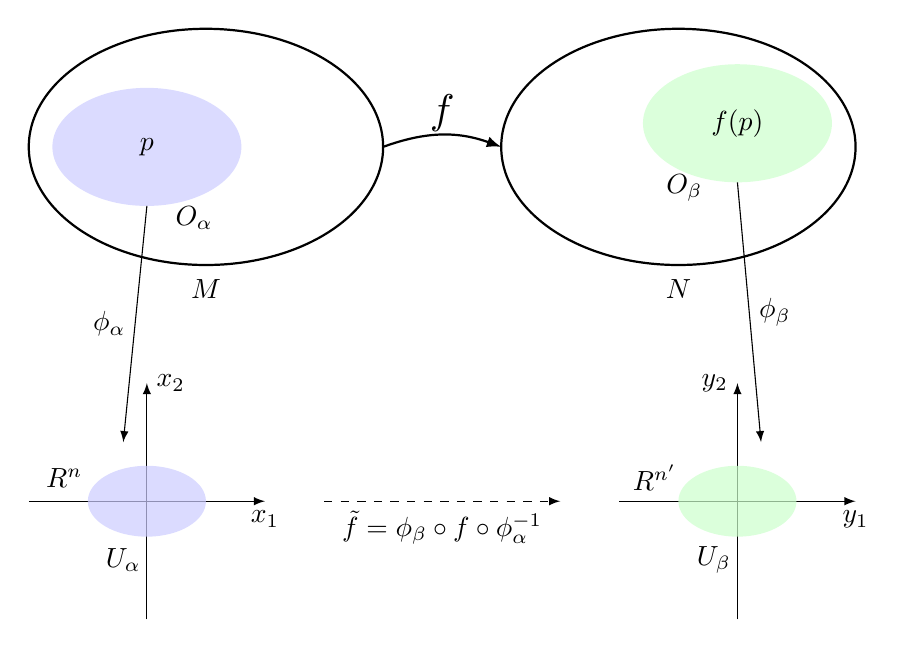
\begin{tikzpicture}[scale=1.5,>=latex]

    % Draw manifold M (as an ellipse) and mark the chart O_alpha
    \draw[thick] (-2,0) ellipse (1.5 and 1);  % Manifold M
    \node at (-2,-1.2) {$M$};  % Label M

    % Draw chart O_alpha as a shaded region on M
    \fill[blue!20,opacity=0.7] (-2.5,0) ellipse (0.8 and 0.5);
    \node at (-2.1,-0.6) {$O_\alpha$};
    \node at (-2.5,0) {$p$};  % Label point p

    % Draw manifold N (as an ellipse) and mark the chart O_beta
    \draw[thick] (2,0) ellipse (1.5 and 1);  % Manifold N
    \node at (2,-1.2) {$N$};  % Label N

    % Draw chart O_beta as a shaded region on N
    \fill[green!20,opacity=0.7] (2.5,0.2) ellipse (0.8 and 0.5);
    \node at (2.05,-0.35) {$O_\beta$};
    \node at (2.5,0.2) {$f(p)$};  % Label point f(p)

    % Draw smooth map f from M to N
    \draw[->, thick] (-0.5,0) to [out=20,in=160] (0.5,0) node[midway,above] {$f$};

    % Add Euclidean spaces R^n and R^{n'}
    %\node at (-2,-2.5) (Rn) {$\mathbb{R}^n$};
    %\node at (2,-2.5) (Rnp) {$\mathbb{R}^{n'}$};

    % Map from O_alpha to R^n
    %\draw[->] (-2.5,-0.6) -- (-2,-2) node[midway,left] {$\phi_\alpha$};

    % Map from O_beta to R^{n'}
    %\draw[->] (2.5,0.5) -- (2,-2) node[midway,right] {$\phi_\beta$};

    % Dashed arrow for the map between R^n and R^{n'}
    %\draw[->, dashed] (Rn) -- (Rnp) node[midway,below] {$\tilde{f} = \phi_\beta \circ f \circ \phi_\alpha^{-1}$};

 % Add Euclidean spaces R^n and R^{n'} as axes
    % R^n axes
    \draw[->] (-3.5,-3) -- (-1.5,-3) node[anchor=north] {$x_1$};
    \draw[->] (-2.5,-4) -- (-2.5,-2) node[anchor=west] {$x_2$};
    \node at (-3.2,-2.8) {$\mathbb{R}^n$};

    % R^{n'} axes
    \draw[->] (1.5,-3) -- (3.5,-3) node[anchor=north] {$y_1$};
    \draw[->] (2.5,-4) -- (2.5,-2) node[anchor=east] {$y_2$};
    \node at (1.8,-2.8) {$\mathbb{R}^{n'}$};

    % Map from O_alpha to R^n
    \draw[->] (-2.5,-0.5) -- (-2.7,-2.5) node[midway,left] {$\phi_\alpha$};

    % Map from O_beta to R^{n'}
    \draw[->] (2.5,-0.3) -- (2.7,-2.5) node[midway,right] {$\phi_\beta$};

    % Dashed arrow for the map between R^n and R^{n'}
    \draw[->, dashed] (-1,-3) -- (1,-3) node[midway,below] {$\tilde{f} = \phi_\beta \circ f \circ \phi_\alpha^{-1}$};

    % Draw open sets U_alpha in R^n and U_beta in R^{n'}
    \fill[blue!20,opacity=0.7] (-2.5,-3) ellipse (0.5 and 0.3);
    \node at (-2.7,-3.5) {$U_\alpha$};

    \fill[green!20,opacity=0.7] (2.5,-3) ellipse (0.5 and 0.3);
    \node at (2.3,-3.5) {$U_\beta$};

\end{tikzpicture}
\end{center}

\begin{remark}
	\begin{itemize}
		\item[]
		\item A smooth map $\psi : M \to N$ which has a smooth inverse is called a \emph{diffeomorphism}\index{diffeomorphism}.
		\item If $N = \mathbb{R}$ or $\mathbb{C}$, we sometimes call $f$ a \emph{scalar field}\index{scalar field}.
		\item If $M = I \subseteq \mathbb{R}$, an open interval, then $f : I \to N$ is a \emph{smooth curve} in $N$.
		\item If $f$ is smooth in one atlas, then it is smooth in all compatible atlases.
	\end{itemize}
\end{remark}

\begin{exbox}
	\begin{enumerate}
		\item Recall $S^1$. Let $f(x, y) = x$, $f : S^1 \to \mathbb{R}$. Using our previous charts,
			\begin{align*}
				f \circ \phi_1^{-1} : (-\pi, \pi) &\to \mathbb{R} \\
				\theta_1 \mapsto \cos \theta_1.
			\end{align*}
			Similarly,
			\begin{align*}
				f \circ \phi_2^{-1} : (0, 2\pi) &\to \mathbb{R} \\
				\theta_2 \mapsto \cos \theta_2.
			\end{align*}
			Hence $f$ is smooth.
		\item If $(O, \phi)$ is a coordinate chart on $M$, write
			\[
			\phi(p) = (x^1(p), x^2(p), \ldots, x^n(p)),
			\]
			for $p \in O$. Then $x^i(p)$ defines a map from $O$ to $\mathbb{R}$. This is smooth for each $i = 1, \ldots, n$. If $(O', \phi')$ is another overlapping coordinate chart, then $x^i \circ (\phi')^{-1}$ is the $i$'th component of $\phi \circ (\phi')^{-1}$, hence smooth.
		\item We can define a smooth function chart-by-chart. For simplicity, let $N = \mathbb{R}$, and let $\{(O_\alpha, \phi_\alpha)\}$ be an atlas on $M$. Define smooth functions
			\[
			F_\alpha : U_\alpha \to \mathbb{R},
			\]
			and suppose that $F_\alpha \circ \phi_\alpha = F_\beta \circ \phi_\beta$ on $O_\alpha \cap O_\beta$, for all $\alpha, \beta$.

			Then for $p \in M$, we can define
			\[
			f(p) = F_\alpha \circ \phi_\alpha(p),
			\]
			for any chart $(O_\alpha, \phi_\alpha)$ with $p \in O_\alpha$. Now $f$ is smooth, as
			\[
			f \circ \phi_p^{-1} = F_\alpha \circ \phi_\alpha \circ \phi_\beta^{-1}.
			\]
			In practice, we often don't distinguish between $f$ and its coordinate chart representations $F_\alpha$.
	\end{enumerate}	
\end{exbox}

\subsection{Curves and Vectors}%
\label{sub:cav}

For a surface in $\mathbb{R}^3$, we have a notion of the `tangent space' at a point $p$, which consists of all vectors tangent to the surface at that point.

The tangent spaces are vector spaces (copies of $\mathbb{R}^2$). Different points have different tangent spaces.

In order to define the tangent space for a manifold, we first consider tangent vectors of a curve.

Recall that $\lambda : I \to M$ a smooth map, is a smooth curve in $M$.

If $\lambda(t)$ is a smooth curve in $\mathbb{R}^n$, and $f : \mathbb{R}^n \to \mathbb{R}$ is a smooth function, the chain rule gives
\[
	\frac{\diff}{\diff t} [f(\lambda(t))] = X(t) \cdot \nabla f(\lambda(t)),
\]
where $X(t) = \diff \lambda / \diff t (t)$ is the tangent vector to $\lambda$ at $t$.

\begin{definition}
	Let $\lambda : I \to M$ be a smooth curve with $\lambda(0) = p$. The \emph{tangent vector}\index{tangent vector} to $\lambda$ at $p$ is the linear map $X_p$ from the space of smooth functions $f : M \to \mathbb{R}$, given by
	\[
	X_p(f) = \frac{\diff}{\diff t} f(\lambda(t)) \biggr|_{t = 0}.
	\]
\end{definition}

We observe that:
\begin{enumerate}[(i)]
	\item $X_p$ is linear: $X_p(f + a g) = X_p(f) + a X_p (g)$, for $f, g$ smooth, and $a \in \mathbb{R}$.
	\item $X_p$ satisfies the Leibniz rule:
		\[
		X_p(fg) = X_p(f) g(p) + f(p) X_p(g).
		\]
\end{enumerate}

If $(O, \phi)$ is a chart and $p \in O$, write
\[
\phi(p) = (x^1(p), \ldots, x^n(p)).
\]
Let $F = f \circ \phi^{-1}$, and $x^i(t) = x^i(\lambda(t))$. Now $F : \mathbb{R}^n \to \mathbb{R}$, and $x : \mathbb{R} \to \mathbb{R}^n$. Then,
\[
f \circ \lambda(t) = f \circ \phi^{-1} \circ \phi \circ \lambda(t) = F \circ x(t),
\]
and by applying the regular chain rule for functions $\mathbb{R}^m \to \mathbb{R}^n$,
\[
\frac{\diff}{\diff t} f(\lambda(t)) \biggr|_{t = 0} = \frac{\partial F}{\partial x^\mu} (x) \cdot \frac{\diff x^\mu}{\diff t} \biggr|_{t = 0}.
\]

% lecture 3

\begin{proposition}
	The set of tangent vectors to curves at $p$ forms a vector space, $T_pM$, of dimension $n = \dim M$. We call $T_p M$ the \emph{tangent space}\index{tangent space} to $M$ at $p$.
\end{proposition}

\begin{proofbox}
	Given $X_p, Y_p$ tangent vectors, we need to show that $\alpha X_p + \beta Y_p$ is a tangent vector for $\alpha, \beta \in \mathbb{R}$.

	Let $\lambda, \kappa$ be smooth curves with $\lambda(0) = \kappa(0) = p$, and whose tangent vectors at $p$ are $X_p, Y_p$, respectively.

	Let $(O, \phi)$ be a chart with $p \in O$ and $\phi(p) = 0$, and define
	\[
	\gamma(t) = \phi^{-1}( \alpha \phi(\lambda (t)) + \beta \phi (\kappa (t)) ).
	\]
	This exists, as this is just the sum of elements in $\mathbb{R}^n$.

	Now $\gamma(0) = \phi^{-1}(0) = p$. If $Z_p$ is the tangent to $v$ at $p$, then
	\begin{align*}
		Z_p(f) &= \frac{\diff}{\diff t} f(v(t)) \biggr|_{t = 0} = \frac{\partial F}{\partial x^\mu} \biggr|_{0} \frac{\diff}{\diff t} [\alpha x^\mu (\lambda(t)) + \beta x^\mu(\kappa(t)) ] \biggr|_{t = 0} \\
		       &= \alpha \frac{\partial F}{\partial x^\mu} \biggr|_0 \frac{\diff}{\diff t} x^\mu(\lambda(t)) \biggr|_{t = 0} + \beta \frac{\partial F}{\partial x^\mu} \biggr|_0 \frac{\diff}{\diff t} x^\mu(\kappa(t)) \biggr|_{t =0} \\
		       &= \alpha X_p(f) + \beta Y_p(f).
	\end{align*}
	Thus $T_p M$ is a vector space.

	To see that $T_p M$ is $n$-dimensional, consider the curves
	\[
		\lambda_\mu(t) = \phi^{-1} \underbrace{(0, \ldots, 0, t, 0, \ldots, 0).}_{\mu\text{'th component}}
	\]
	We denote the tangent vector to $\lambda_\mu$ at $p$ by $(\partial / \partial x^\mu)_p$. To see why, note that
	\[
	\left(\frac{\partial}{\partial x^\mu} \right)_p f = \frac{\partial F}{\partial x^\mu} \biggr|_{\phi(p) = 0}.
	\]

	These vectors are linearly independent. Otherwise there exists $\alpha^\mu$ not all zero such that
	\[
	\alpha^\mu \left( \frac{\partial}{\partial x^\mu} \right)_p = 0 \implies \alpha^\mu \frac{\partial F}{\partial x^\mu} \biggr|_0 = 0,
	\]
	for all $F$. Setting $F = x^\nu$ gives $\alpha^\nu = 0$.

	Further, these vectors form a basis for $T_p M$, since if $\lambda$ is any curve with tangent $X_p$ at $p$, then
	\[
	X_p(f) = \frac{\partial F}{\partial x^\mu} \biggr|_0 \frac{\diff}{\diff t} x^\mu(\lambda(t)) \biggr|_{t = 0} = X^\mu \left( \frac{\partial}{\partial x^\mu} \right) f.
	\]
	Here, we set
	\[
	X^\mu = \frac{\diff}{\diff t} x^\mu(\lambda(t)) \biggr|_{t = 0}.
	\]
	These are the components of $X_p$ with respect to the basis.
\end{proofbox}

\begin{center}
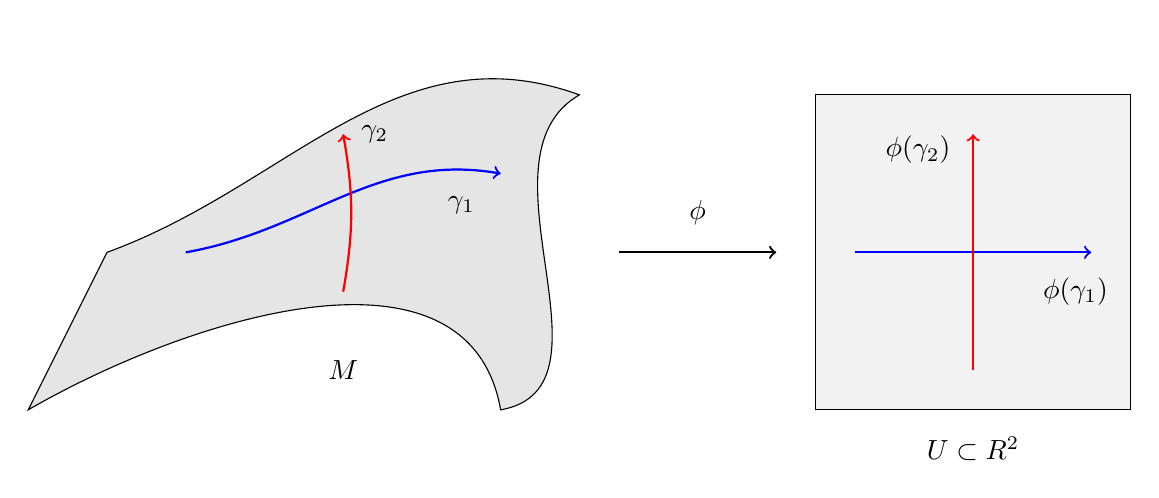
\begin{tikzpicture}

% Manifold M (2D surface, wavy shape)
\draw[fill=gray!20] (0,0) to[out=20,in=160] (6,2) to[out=-150,in=10] (5,-2) to[out=100, in=30] (-1, -2) -- cycle;
\node at (3, -1.5) {$M$};

% Horizontal path on M (blue)
\draw[thick, blue, ->] (1,0) to[out=10,in=170] (5,1);
\node at (4.5, 0.6) {$\gamma_1$};

% Vertical path on M (red)
\draw[thick, red, ->] (3,-0.5) to[out=80,in=-80] (3,1.5);
\node at (3.4, 1.5) {$\gamma_2$};

% Projection map phi
\draw[->, thick] (6.5,0) -- (8.5,0);
\node at (7.5, 0.5) {$\phi$};

% Open set U in R^2 (rectangle)
\draw[fill=gray!10] (9, 2) rectangle (13, -2);
\node at (11, -2.5) {$U \subset \mathbb{R}^2$};

% Projection of horizontal path in U
\draw[thick, blue, ->] (9.5,0) -- (12.5,0);
\node at (12.3, -0.5) {$\phi(\gamma_1)$};

% Projection of vertical path in U
\draw[thick, red, ->] (11,-1.5) -- (11,1.5);
\node at (10.3, 1.3) {$\phi(\gamma_2)$};

% Axes in U (x and y)
%\draw[->] (9,-4.5) -- (9,-0.5) node[anchor=south east] {$y$};
%\draw[->] (9,-4.5) -- (13,-4.5) node[anchor=north west] {$x$};

\end{tikzpicture}
\end{center}

Notice that the basis $\{(\partial / \partial x^\mu)_p\}$ depends on the coordinate chart $\phi$. Suppose we choose another chart $(O', \phi')$, again centred at $p$. Write $\phi' = (x'^1, \ldots, x'^n)$.

Then if $F\ = f \circ (\phi')^{-1}$, then
\begin{align*}
	F(x) & = f \circ \phi^{-1}(x) = f \circ (\phi')^{-1} \circ \phi' \circ \phi^{-1}(x)  \\
	     &= F'(x'(x)).
\end{align*}
Therefore,
\[
	\left( \frac{\partial}{\partial x^\mu} \right)_p f = \frac{\partial F}{\partial x^\mu} \biggr|_{\phi(p)} = \left( \frac{\partial x'^\nu}{ \partial x^\mu} \right)_{\phi(p)} \left( \frac{\partial F'}{\partial x'^\nu} \right)_{\phi'(p)} = \left( \frac{\partial x'^\nu}{ \partial x^\mu} \right)_{\phi(p)} \cdot \left( \frac{\partial}{\partial x'^\nu} \right)_p f.
\]
We deduce that
\[
\left( \frac{\partial}{\partial x^\mu} \right)_p = \left( \frac{\partial x'^\nu}{\partial x^\mu}\right)_{\phi(p)} \left( \frac{\partial}{\partial x'^\nu} \right)_p.
\]
So let $X^\mu$ be the components of $X_p$ with respect to $\{(\partial / \partial x^\mu)_p\}$, and $X'^\mu$ be the components with respect to $\{(\partial / \partial x'^\mu)_p\}$. So,
\begin{align*}
	X_p &= X^\mu \left( \frac{\partial}{\partial x^\mu} \right)_p = X'^\mu \left( \frac{\partial}{\partial x'^\mu} \right)_p \\
	    &= X^\mu \left( \frac{\partial x'^\sigma}{\partial x^\mu} \right)_{\phi(p)} \left( \frac{\partial}{\partial x'^\sigma} \right)_p.
\end{align*}
Therefore,
\[
X'^\mu = \left( \frac{\partial x'^\mu}{\partial x^\nu} \right)_{\phi(p)} X^\nu.
\]
We do not have to choose a coordinate basis such as $\{(\partial/\partial x^\mu)_p\}$. With respect to a general basis $\{e_\mu\}$ for $T_p M$, we write $X_p = X^\mu e_\mu$, for $X^\mu \in \mathbb{R}$ the components.

We always use summation conventions: we always contract one upstairs and one downstairs index.

\subsection{Covectors}%
\label{sub:cov}

Recall that if $V$ is a vector space over $\mathbb{R}$, the \emph{dual space}\index{dual space} $V^\ast$ is the space of linear maps from $V$ to $\mathbb{R}$. If $V$ is $n$-dimensional, then so is $V^\ast$.

Given a basis $\{e_\mu\}$ for $V$, we define the \emph{dual basis}\index{dual basis} $\{f^\mu\}$ for $V^\ast$ by requiring that
\[
f^\mu(e_\nu) = \delta\indices{^{\mu}_{\nu}}.
\]
If $V$ is finite dimensional, then $V^{\ast\ast} = (V^\ast)^\ast$ is isomorphic to $V$: to an element $x$ of $V$, we assign a linear map $\Lambda_x : V^\ast \to \mathbb{R}$ by
\[
\Lambda_x(\omega) = \omega(x).
\]
\begin{definition}
	The dual space of $T_pM$ is denoted $T^\ast_p M$, and is called the \emph{cotangent space}\index{cotangent space} to $M$ at $p$.

	An element of this space is a covector at $p$. If $\{e_\mu\}$ is a basis for $T_p M$ and $\{f^\mu\}$ the dual basis for $T^\ast_p M$, then we can expand a covector $\eta$ as
	\[
	\eta = \eta_\mu f^\mu,
	\]
	for $\eta_\mu \in \mathbb{R}$ the components of $\eta$.
\end{definition}

% lecture 4

Note that:
\begin{itemize}
	\item $\eta(e_\nu) = \eta_\mu f^\mu (e_\nu) = \eta_\mu \delta\indices{^{\mu}_{\nu}} = \eta_\nu$.
	\item $\eta(X) = \eta(X^\mu e_\mu) = X^\mu \eta(e_\mu) = X^\mu \eta_\mu$.
\end{itemize}

\begin{definition}
	If $f : M \to \mathbb{R}$ is a smooth function, define $(\diff f)_p \in T^\ast_p M$, the \emph{differential}\index{differential} of $f$ at $p$, by
	\[
		(\diff f)_p (X) = X(f),
	\]
	for any $X \in T_p M$. $(\diff f)_p$ is sometimes also called the \emph{gradient}\index{gradient} of $f$ at $p$.
\end{definition}

If $f$ is a constant, then $X(f) = 0 \implies (\diff f)_p = 0$.

If $(O, \phi)$ is a coordinate chart with $p \in O$ and $\phi = (x^1, \ldots, x^n)$, then we can set $f = x^\mu$ to find $(\diff x^\mu)_p$. Now,
\[
	(\diff x^\mu)_p \left( \frac{\partial}{\partial x^\nu} \right)_p = \left( \frac{\partial x^\mu}{\partial x^\nu} \right)_{\phi(p)} = \delta\indices{^{\mu}_{\nu}}.
\]
Hence, $\{(\diff x^\mu)_p\}$ is the dual basis to $\{(\partial/\partial x^\mu)_p\}$. In this basis, we can compute
\[
	[(\diff f)_p]_\mu = (\diff f)_p \left( \frac{\partial}{\partial x^\mu} \right)_p = \left( \frac{\partial}{\partial x^\mu} \right)_p f = \left( \frac{\partial F}{\partial x^\mu} \right)_{\phi(p)},
\]
justifying the language of the `gradient'.

It can be shown that if $(O', \phi')$ is another chart with $p \in O'$, then
\[
	(\diff x^\mu)_p = \left( \frac{\partial x^\mu}{\partial x'^\nu} \right)_{\phi'(p)} (\diff x'^\nu)_p,
\]
where $x(x') = \phi \circ \phi'^{-1}$, and hence if $\eta_\mu$, $\eta'_\mu$ are components with respect to these bases, then
\[
\eta_\mu' = \left(\frac{\partial x^\nu}{\partial x'^\mu} \right)_{\phi'(p)} \eta_\nu.
\]

\subsection{The (Co)tangent bundle}%
\label{sub:tb}

We can glue together the tangent spaces $T_pM$ as $p$ varies to get a new $2n$ dimensional manifold, $TM$, the \emph{tangent bundle}\index{tangent bundle}. We let
\[
	TM = \bigcup_{p \in M} \{p\} \times T_pM,
\]
the set of ordered pairs $(p, X)$, with $p \in M$, $X \in T_pM$. If $\{(O_\alpha, \phi_\alpha)\}$ is an atlas on $M$, we obtain an atlas for $TM$ by setting
\[
	\tilde O_\alpha = \bigcup_{p \in O_\alpha} \{p\} \times T_p M,
\]
and
\[
\tilde \phi_\alpha((p, X)) = (\phi_\alpha(p), X^\mu) \in U_\alpha \times \mathbb{R}^{n} = \tilde U_\alpha,
\]
where $X^\mu$ are the components of $X$ with respect to the coordinate basis of $\phi_\alpha$.

It can be shown that if $(O, \phi)$ and $(O', \phi')$ are two charts on $M$, on $\tilde U \cap \tilde U'$, if we write $\phi' \circ \phi^{-1}(x) = x'(x)$, then
\[
\tilde \phi' \circ \tilde \phi^{-1}(x, X^\mu) = \left( x'(x), \frac{\partial x'^\mu}{\partial x^\nu} X^\nu \right).
\]
This lets us deduce that $TM$ is a manifold.

A similar construction permits us to define the \emph{cotangent bundle}\index{cotangent bundle}
\[
	T^\ast M = \bigcup_{p \in M} \{p\} \times T_p^\ast M.
\]
The map $\pi : TM \to M$ which takes $(p, X) \mapsto p$ is smooth (show this!)

\subsection{Abstract Index Notation}%
\label{sub:ain}

We have used Greek letters $\mu, \nu$ to label components of vectors (or covectors) with respect to the bases $\{e_\mu\}$. Equations involving these quantities refer to the specific basis, for example if we write $X^\mu = \delta^\mu$, this says $X$ only has one non-zero component \emph{in the current basis}, which will not be true in other bases.

However, we know that some equations hold in all bases, e.g.
\[
\eta(X) = X^\mu \eta_\mu.
\]
To capture this, we can use \emph{abstract index notation}\index{abstract index notation}. We denote a vector by $X^a$, where the latin index $a$ does not denote a component, rather it tells us that $X^a$ is a vector. Similarly we denote a covector $\eta$ by $\eta_a$.

If an equation is true in all bases, then we can replace Greek indices by latin indices:
\[
\eta(X) = X^a \eta_a = \eta_a X^a,
\]
or
\[
X(f) = X^a (\diff f)_a.
\]
An equation in abstract index notation can always be turned into an equation for components, by picking a basis and changing $a \to \mu$, $b \to \nu$.

\subsection{Tensors}%
\label{sub:tens}

In Newtonian physics, we know that some quantities are described by higher rank orders, e.g. the inertia tensor or the metric.

\begin{definition}
	A \emph{tensor}\index{tensor} of type $(r, s)$ is a multilinear map
	\[
		T : (T^\ast_p M)^r \times (T_p M)^s \to \mathbb{R}.
	\]
\end{definition}

\begin{exbox}
	\begin{enumerate}
		\item A tensor of type $(0, 1)$ is a linear map $T_p M \to \mathbb{R}$, i.e. just a covector.
		\item A tensor of type $(1, 0)$ is a linear map $T^\ast p M \to \mathbb{R}$, i.e. an element of $(T^\ast p M)^\ast \cong T_p M$, a vector.
		\item We can define a $(1, 1)$ tensor $\delta$ by
			\[
			\delta(\omega, X) = \omega(X),
			\]
		where $\omega \in T_p^\ast M$, $X \in T_p M$.
	\end{enumerate}
\end{exbox}

If $\{e_\mu\}$ is a basis for $T_p M$ and $\{f^\mu\}$ its dual basis, then the components of an $(r, s)$ tensor $T$ are
\[
T\indices{^{\mu_1 \cdots \mu_r}_{\nu_1 \cdots \nu_s}} = T(f^\mu_1, \ldots, f^{\mu_r}, e_{\nu_1}, \ldots, e_{\nu_s}).
\]
In abstract index notation, we denote $T$ by $T\indices{^{a_1 \cdots a_r}_{b_1 \cdots b_s}}$. Tensors at $p$ form a vector space over $\mathbb{R}$ of dimension $n^{r + s}$.

\begin{exbox}
	\begin{enumerate}
		\item Consider $\delta$ above. Then,
			\[
			\delta\indices{^{\mu}_{\nu}} = \delta(f^\mu, e_\nu) = f^\mu(e_\nu) =
			\begin{cases}
				1 & \mu = \nu,\\
				0 & \mu \neq \nu.
			\end{cases}
			\]
			We can write $\delta$ as $\delta\indices{^{a}_{b}}$ in AIN.
		\item Consider a $(2, 1)$ tensor $T$, and let $\omega, \eta \in T_p^\ast M$, $X \in T_p M$. Then,
			\begin{align*}
				T(\omega, \eta, X) &= T(\omega_\mu f^\mu, \eta_\nu f^\nu, X^\sigma e_\sigma) \\
						   &= \omega_\mu \eta_\nu X^\sigma T(f^\mu, f^\nu, e_\sigma) \\
						   &= \omega_\mu \eta_\nu X^\sigma T\indices{^{\mu\nu}_{\sigma}}.
			\end{align*}
			In AIN,
			\[
			T(\omega, \nu, X) = \omega_a \eta_b X^c T\indices{^{ab}_{c}}.
			\]
			This can be generalized to higher ranks.
	\end{enumerate}
	
\end{exbox}

% lecture 5

\subsection{Change of Bases}%
\label{sub:cob}

We have already seen how the components of $X$ or $\eta$ with respect to a coordinate basis ($X^\mu, \eta_\nu$ respectively) change under a change of coordinates.

But we do not only have to consider coordinate bases.

Suppose $\{e_\mu\}$ and $\{e'_\mu\}$ are two bases for $T_pM$ with dual bases $\{f^\mu\}$ and $\{f'^\mu\}$.

As these are bases, we can expand
\[
f'^\mu = A\indices{^{\mu}_{\nu}} f^\nu, \qquad e'_\mu = B\indices{^{\nu}_{\mu}} e_\nu,
\]
for some $A\indices{^{\mu}_{\nu}}, B\indices{^{\mu}_{\nu}} \in \mathbb{R}$. But,
\begin{align*}
	\delta\indices{^{\mu}_{\nu}} &= f'^\mu (e'_\nu) = A\indices{^{\mu}_{\tau}} f^\tau ( B\indices{^{\sigma}_{\nu}} e_\sigma) \\
				     &= A\indices{^{\mu}_{\tau}} B\indices{^{\sigma}_{\nu}} f^\tau(e_\sigma) = A\indices{^{\mu}_{\tau}} B\indices{^{\sigma}_{\nu}} \delta\indices{^{\tau}_{\sigma}} \\
				     &= A\indices{^{\mu}_{\sigma}} B\indices{^{\sigma}_{\nu}}.
\end{align*}
Therefore, looking at these as matrices,
\[
B\indices{^{\mu}_{\nu}} = (A^{-1})\indices{^{\mu}_{\nu}}.
\]
If
\[
e_\mu = \left( \frac{\partial}{\partial x^\mu} \right)_p, \qquad e'_\mu = \left( \frac{\partial}{\partial x'^\mu} \right)_p,
\]
then we have already seen
\[
A\indices{^{\mu}_{\nu}} = \left( \frac{\partial x'^\mu}{\partial x^\nu} \right)_{\phi(p)}, \qquad B\indices{^{\mu}_{\nu}} = \left( \frac{\partial x^\mu}{\partial x'^\nu} \right)_{\phi(p)},
\]
which indeed satisfies $A\indices{^{\mu}_{\sigma}}B\indices{^{\sigma}_{\nu}} = \delta\indices{^{\mu}_{\nu}}$, by the chain rule.

A chance of bases induces a transformation of tensor components, for example if $T$ is a $(1, 1)$-tensor, then
\begin{align*}
	T\indices{^{\mu}_{\nu}} &= T(f^\mu, e_\nu) \\
	{T'}\indices{^{\mu}_{\nu}} &= T(f'^\mu, e'_\nu) = T(A\indices{^{\mu}_{\sigma}} f^\sigma, (A^{-1})\indices{^{\tau}_{\nu}} e_\tau ) \\
				 &= A\indices{^{\mu}_{\sigma}} (A^{-1})\indices{^{\tau}_{\nu}} T(f^\sigma, e_\tau) \\
				 &= A\indices{^{\mu}_{\sigma}} (A^{-1})\indices{^{\tau}_{\nu}} T\indices{^{\sigma}_{\tau}}.
\end{align*}


\subsection{Tensor Operations}%
\label{sub:top}

Given an $(r, s)$-tensor, we can form a $(r - 1, s-1)$-tensor by \emph{contraction}\index{contraction}.

For simplicity, assume $T$ is a $(2, 2)$-tensor. Define a $(1, 1)$-tensor $S$ by
\[
S(\omega, X) = T(\omega, f^\mu, X, e_\mu).
\]
To see that this is independent of the choice of basis, note
\begin{align*}
	T(\omega, f'^\mu, X, e'_\mu) &= T(\omega, A\indices{^{\mu}_{\sigma}} f^\sigma, X, (A^{-1})\indices{^{\tau}_{\mu}} e_\tau ) = A\indices{^{\mu}_{\sigma}} (A^{-1})\indices{^{\tau}_{\mu}} T(\omega, f^\sigma, X, e_\tau) \\
				     &= \delta\indices{^{\tau}_{\sigma}} T(\omega, f^\sigma, X, e_\tau) = T(\omega, f^\tau, X, e_\tau) = S(\omega, X).
\end{align*}
So this does not depend on the choice of basis. $S$ and $T$ have components related by
\[
S\indices{^{\mu}_{\nu}} = T\indices{^{\mu\sigma}_{\nu\sigma}}.
\]
In any basis in AIN we write
\[
S\indices{^{a}_{b}} = T\indices{^{ac}_{bc}}.
\]
We can generalise to contract any upstairs index with any downstairs index in a general $(r, s)$-tensor.

Another way to make new tensors from old tensors is to form the \emph{tensor product}\index{tensor product}. If $S$ is a $(p, q)$-tensor and $T$ is a $(r, s)$-tensor, then $S \otimes T$ is an $(p + r, q + s)$-tensor:
\begin{align*}
	S \otimes &T(\omega^1, \ldots, \omega^p, \eta^1, \ldots, \eta^r, X_1, \ldots, X_q, Y_1, \ldots, Y_s) \\
		  &= S(\omega^1, \ldots, \omega^p, X_1, \ldots, X_q) T(\eta^1, \ldots, \eta^r, Y_1, \ldots, Y_s).
\end{align*}
This is independent of basis. In AIN,
\[
	(S \otimes T)\indices{^{a_1\ldots a_p b_1 \ldots b_r}_{c_1 \ldots c_q d_1 \ldots, d_s}} = S\indices{^{a_1 \ldots a_r}_{ c_1 \ldots c_q}} T\indices{^{b_1 \ldots b_r}_{d_1 \ldots b_r}}.
\]
We can show that for any $(1, 1)$-tensor $T$, in any basis we have
\[
T = T\indices{^{\mu}_{\nu}} e_\mu \otimes f^\nu.
\]
The final tensor operations we require are \emph{(anti)symmetrization}\index{symmetrization}\index{antisymmetrization}. If $T$ is a $(0, 2)$-tensor, we can define two new tensors:
\begin{align*}
	S(X, Y) &= \frac{1}{2}(T(X, Y) + T(Y, X)), \\
	A(X, Y) &= \frac{1}{2} (T(X, Y) - T(Y, X)).
\end{align*}
In AIN,
\begin{align*}
	S_{ab} = \frac{1}{2} (T_{ab} + T_{ba}) = T_{(ab)}, \\
	A_{ab} = \frac{1}{2} (T_{ab} - T_{ba}) = T_{[ab]}.
\end{align*}
These operations can be applied to any pair of matching symmetries in a more general tensor, for example:
\[
T\indices{^{a(bc)}_{de}} = \frac{1}{2} (T\indices{^{abc}_{de}} + T\indices{^{acb}_{de}}).
\]
We can also (anti)symmetrize over more than two indices.
\begin{itemize}
	\item To symmetrize over $n$ indices, we sum over all permutations of the indices and divide by $n!$.
	\item To anti-symmetrize over $n$ indices, we sum over all permutation weighted by their sign, and then divide by $n!$.
\end{itemize}

For example,
\begin{align*}
	T^{(abc)} &= \frac{1}{3!} (T^{abc} + T^{bca} + T^{cab} + T^{acb} + T^{cba} + T^{bac}), \\
	T^{[abc]} &= \frac{1}{3!} (T^{abc} + T^{bca} + T^{cab} - T^{acb} - T^{cba} - T^{bac}.
\end{align*}
To exclude indices from (anti)symmetrization, we use vertical lines:
\[
T^{(a|b|c)} = \frac{1}{2} (T^{abc} + T^{c b a}).
\]
\subsection{Tensor Bundles}%
\label{sub:tense_buns}

The space of $(r, s)$-tensors at a point $p$ is the vector space $(T\indices{^{r}_{s}})_pM$. These can be glued together to form the bundle of $(r, s)$-tensors
\[
	T\indices{^{r}_{s}} M = \bigcup_{p \in M}\{ p\} \times (T\indices{^{r}_{s}} )_p M.
\]
If $(O, \phi)$ is a coordinate chart on $M$, set
\[
	\tilde O = \bigcup_{p \in O} \{p\} \times (T^{\indices{^{r}_{s}}})_p M \subseteq T\indices{^{r}_{s}}M,
\]
and
\[
\tilde \phi(p, S_p) = (\phi(p), S\indices{^{\mu_1 \ldots \mu_r}_{\nu_1 \ldots \nu_s}} ).
\]
$T\indices{^{r}_{s}} M$ is a manifold, with a natural smooth map $\Pi : T\indices{^{r}_{s}}M \to M$ such that $\pi(p, S_p) = p$.

A \emph{tensor field}\index{tensor field} is a smooth map $T : M \to T\indices{^{r}_{s}}M$ such that $\pi \circ T = \id$.

If $(O, \phi)$ is a coordinate chart on $M$, then
\[
\tilde \phi \circ T \circ \phi(x) = (x, T\indices{^{\mu_1 \ldots \mu_r}_{ \nu_1 \ldots \nu_s}}(x)),
\]
which is smooth provided the components $T\indices{^{\mu_1 \ldots, \mu_r}_{ \nu_1 \ldots \nu_s}}(x)$ are smooth functions of $x$.

\begin{exbox}
	If $T\indices{^{r}_{s}} M = T\indices{^{1}_{0}}M \cong TM$, the tensor field is called a \emph{vector field}\index{vector field}. In a local coordinate patch, if $X$ is a vector field, we write $X(p) = (p, X_p)$, with
	\[
	X_p = X^\mu(x) \left( \frac{\partial}{\partial x^\mu} \right)_p.
	\]
	In particular, $\partial / \partial x^\mu$ are always smooth, but only defined locally.
\end{exbox}

% lecture 6

A vector field can act on a function $f : M \to \mathbb{R}$ to give a new function $Xf$ by
\[
Xf(p) = X_p(f).
\]
In coordinates,
\[
Xf(p) = X^\mu(\phi(p)) \frac{\partial F}{\partial x^\mu} \biggr|_{\phi(p)},
\]
where $F = f \circ \phi^{-1}$.

\subsection{Integral Curves}%
\label{sub:ic}

Given a vector field $X$ on $M$, we say a curve $\lambda : I \to M$ is an \emph{integral curve}\index{integral curve} of $X$ if its tangent at every point $x$, which we denote by $\diff \lambda/ \diff t$, then
\[
\frac{\diff \lambda}{\diff t} (t) = X_{\lambda(t)}.
\]
Through each point $p$, there is a unique integral curve passing through it, unique up to extension or shift of the parameter.

To see this, pick a chart $\phi$ with $\phi = (x^1, \ldots, x^n)$, and $\phi(p) = 0$. In this chart, the equation becomes
\[
\frac{\diff x^\mu}{\diff t}(t) = X^\mu(x(t)),
\]
where $x^\mu(t) = x^\mu(\lambda(t))$. Assuming without loss of generality that $\lambda(0) = p$, we get an initial condition $x^\mu(0)= 0$.

By standard ODE theory, this equation with initial conditions has a solution which is unique up to extension.

\subsection{Commutators}%
\label{sub:com}

Suppose $X$ and $Y$ are two vector fields, and $f : M \to \mathbb{R}$ is smooth. Then $X(Y(f))$ is a smooth function, however it is not of the form $K(f)$ for some vector field $K$, since
\begin{align*}
	X(Y(fg)) &= X(f Y(g) + g Y(f)) = X(f(Y(g)) + X(g Y(f)) \\
		 &= f X(Y(g)) + g X(Y(f)) + X(f) Y(g) + X(g) Y(f).
\end{align*}
So the Leibniz rule does not hold. But, if we consider $[X, Y](f) = X(Y(f)) - Y(X(f))$, then the Leibniz rule does hold. In fact, $[X, Y]$ defines a vector field.

To see this, we can use coordinates:
\begin{align*}
	[X, Y](f) &= X \left( Y^\nu \frac{\partial f}{\partial x^\nu} \right) - Y \left( X^\mu \frac{\partial f}{\partial x^\mu} \right) \\
		  &= X^\mu \frac{\partial}{\partial x^\mu} \left( Y^\nu \frac{\partial f}{\partial x^\nu} \right) - Y^\nu \frac{\partial}{\partial x^\nu} \left( X^\mu \frac{\partial F}{\partial x^\mu} \right) \\
		  &= X^\mu Y^\nu \left( \frac{\partial^2 f}{\partial x^\mu \partial x^\nu} - \frac{\partial^2 f}{\partial x^\nu \partial x^\mu} \right) + X ^\mu \frac{\partial Y^\nu}{\partial x^\mu} \frac{\partial F}{\partial x^\nu} - Y^\nu \frac{\partial X^\mu}{\partial x^\nu} \frac{\partial F}{\partial x^\mu} \\
		  &= \left( X^\mu \frac{\partial Y^\nu}{\partial x^\mu} - Y^\mu \frac{\partial X^\nu}{\partial x^\mu} \right) \frac{\partial F}{\partial x^\nu} \\
		  &= [X, Y]^\nu \frac{\partial F}{\partial x^\nu},
\end{align*}
where
\[
	[X, Y]^\nu = X^\mu \frac{\partial Y^\nu}{\partial x^\mu} - Y^\mu \frac{\partial X^\nu}{\partial x^\mu}
\]
are the components of the commutator. Since $f$ is arbitrary,
\[
	[X, Y] = [X, Y]^\nu \frac{\partial}{\partial x^\nu}
\]
is valid only in a coordinate basis.

\subsection{Metric Tensor}%
\label{sub:met_tens}

We are familiar from Euclidean geometry (and special relativity) with the fact that the fundamental object when talking about distances and angles (or time intervals and rapidity) is an inner product between vectors. For example,
\[
\mathbf{x} \cdot \mathbf{y} = x_1 y_1 + x_2 y_2 + x_3 y_3
\]
in $\mathbb{R}^3$ with Euclidean geometry, and
\[
	X \cdot Y = - X^0 Y^0 + X^1 Y^1 + X^2 Y^2 + X^3 Y^3
\]
for $\mathbb{R}^{3 + 1}$ with the Minkowski geometry (and $c = 1$).

\begin{definition}
	A \emph{metric tensor}\index{metric tensor} at $p \in M$ is a $(0, 2)$-tensor satisfying:
	\begin{enumerate}[(i)]
		\item $g$ is symmetric, so $g(X, Y) = g(Y, X)$ for all $X, Y \in T_pM$. In coordinates, $g_{ab} = g_{ba}$.
		\item $g$ is \emph{non-degenerate}\index{non-degenerate}: $g(X, Y) = 0$ for all $Y \in T_p M$ if and only if $X = 0$.
	\end{enumerate}
\end{definition}

We sometimes write
\[
g(X, Y) = \langle X, Y\rangle = \langle X, Y\rangle_g = X \cdot Y.
\]
By adapting the Gram-Schmidt algorithm, we can always find a basis $\{e_\mu\}$ for $T_p M$ such that
\[
g(e_\mu, e_\nu) =
\begin{cases}
	0 & \mu \neq \nu, \\
	+1 \text{ or } -1 & \mu = \nu.
\end{cases}
\]
The number of $-1$'s and $1$'s does not depend on the choice of basis, by Sylvester's law of inertia, and is called the \emph{signature}\index{signature}.

If $g$ has signature that is entirely positive, we say it is \emph{Riemannian}\index{Riemannian}.

If $g$ has signature that is positive apart from one component, we say it is \emph{Lorentzian}\index{Lorentzian}.

\begin{definition}
	A \emph{Riemannian} (resp. \emph{Lorentzian}) manifold is a pair $(M, g)$ where $M$ is a manifold, and $g$ is a Riemannian (resp. Lorentzian) metric tensor field.

	On a Riemannian manifold, the \emph{norm}\index{norm} of a vector $X \in T_p M$ is
	\[
		|X| = \sqrt{g(X, X)},
	\]
	and the \emph{angle}\index{angle} between $X, Y \in T_p M$ is given by
	\[
	\cos \theta = \frac{g(X, Y)}{|X||Y|}.
	\]
	The \emph{length}\index{length} of a curve $\lambda : (a, b) \to M$ is given by
	\[
	\ell(\lambda) = \int_a^b \left| \frac{\diff \lambda}{\diff t} (t) \right| \diff t.
	\]
\end{definition}

It is an easy exercise to show that if $\tau : (c, d) \to (a, b)$ is a reparametrization with $\diff \tau/ \diff u > 0$, and $\tau(c) = a$, $\tau(d) = b$, then $\tilde \lambda = \lambda \circ \tau : (c, d) \to M$ is a reparametrization of $\lambda$, in which $\ell(\tilde \lambda) = \ell(\lambda)$.

% lecture 7

In a coordinate basis, $g = g_{\mu\nu} \diff x^\mu \otimes \diff x^\nu$. We often write
\[
\diff x^\mu \diff x^\nu = \frac{1}{2} (\diff x^\mu \otimes \diff x^\nu + \diff x^\nu \otimes \diff x^\mu).
\]
And by convention we often write $g = \diff s^2$, so that
\[
g = \diff s^2 = g_{\mu\nu} \diff x^\mu \diff x^\nu.
\]
\begin{exbox}
	\begin{enumerate}[(i)]
		\item Consider $\mathbb{R}^n$ with
			\[
			g = \diff s^2 = (\diff x^1)^2 + (\diff x^2)^2 + (\diff x^n)^2 + \delta_{\mu\nu} \diff x^\mu \diff x^\nu.
			\]
			This is called Euclidean space, and any chart covering $\mathbb{R}^n$ in which the metric takes this form is called \emph{Cartesian}\index{Cartesian}.
		\item Consider $\mathbb{R}^{1+3}$ with
			\[
			g = \diff s^2 = -(\diff x^0)^2 + (\diff x^1)^2 + (\diff x^2)^2 + (\diff x^3)^2 = \eta_{\mu\nu} \diff x^\mu \diff x^\nu.
			\]
			This is \emph{Minkowski space}\index{Minkowski space}. A coordinate chart covering $\mathbb{R}^{1+3}$ in which the metric takes this form is an \emph{intertial frame}\index{intertial frame}.
		\item On $S^2 = \{\mathbf{x} \in \mathbb{R}^3 \mid |\mathbf{x}| = 1\}$, define a chart by $\phi^{-1} : (0, \pi) \times (-\pi, \pi) \to S^2$ by
			\[
				(\theta, \varphi) \mapsto (\sin\theta \cos \varphi, \sin \theta \sin \varphi, \cos \theta).
			\]
			In this chart, the round metric is
			\[
			g = \diff s^2 = \diff \theta^2 + \cos^2\theta \diff \varphi^2.
			\]
			This covers $S^2 \setminus \{\mathbf{x}| = 1, x^2 = 0, x^1 \leq 0\}$.

			To cover the rest, let $\tilde \phi^{-1}$ be given by
			\[
				(\theta', \varphi') \mapsto (-\sin\theta' \cos \varphi', \cos \theta', \sin \theta' \sin \varphi').
			\]
			Setting $g = \diff \theta'^2 + \sin^2 \theta' \diff \varphi'^2$ defines a metric on all of $S^2$.
	\end{enumerate}
\end{exbox}

Since $g_{ab}$ is non-degenerate, it is invertible as a matrix in any basis. We can check the inverse define a symmetric $(2, 0)$-tensor $g^{ab}$ satisfying
\[
g^{ab} g_{bc} = \delta\indices{^{a}_{c}}.
\]

\begin{exbox}
	In the $\phi$ coordinates of the $S^2$ example, note
	\[
	g^{\mu\nu} = \left( 1, \frac{1}{\sin^2\theta}\right).
	\]
\end{exbox}

An important property of the metric is that it induces a canonical identification of $T_pM$ and $T^\ast_pM$.

Given $X^a \in T_pM$, we define a covector $g_{ab} X^b = X_a$, and given $\eta_a \in T_p^\ast M$, we define a vector $g^{ab}\eta_b = \eta^a$.

In $(\mathbb{R}^3, \delta)$ we often do this without realizing. More generally, this allows us to raise tensor indices with $g^{ab}$ and lower with $g_{ab}$. For example if $T\indices{^{ab}_{c}}$ is  $(2, 1)$-tensor, then $T\indices{_{a}^{bc}}$ is the $(2, 1)$-tensor given by
\[
T\indices{_{a}^{bc}} = g_{ad} g^{ce} T\indices{^{db}_{e}}.
\]

\subsection{Lorentzian Signature}%
\label{sub:lorsig}

In Lorentzian signature, with indices $0, 1, \ldots, n$. At any point in a Lorentzian manifold we can find a basis $\{e_\mu\}$ such that
\[
g(e_\mu, e_\nu) = \eta_{\mu\nu} = \mathrm{diag}(-1, 1, 1, \ldots, 1).
\]
This basis is not unique; if $e_\mu' = (A^{-1})\indices{^{\nu}_{\mu}} e_\nu$ is another such basis, then
\[
\eta_{\mu\nu} = g(e_\mu', e_\nu') = (A^{-1})\indices{^{\sigma}_{\mu}} (A^{-1})\indices{^{\tau}_{\nu}} g(e_\sigma, e_\tau) = (A^{-1})\indices{^{\sigma}_{\mu}} (A^{-1})\indices{^{\tau}_{\nu}} \eta_{\sigma\tau}.
\]
This is the condition that $A$ is a \emph{Lorentz transformation}\index{Lorentz transformation}.

The tangent space at $p$ has $\eta_{\mu\nu}$ as a metric tensor, so it has the structure of Minkowski space.

\begin{definition}
	$X \in T_p M$ is:
	\begin{itemize}
		\item \emph{spacelike}\index{spacelike} if $g(X, X) > 0$,
		\item \emph{null}\index{null} or \emph{lightlike}\index{lightlike} if $g(X, X) = 0$,
		\item \emph{timelike}\index{timelike} if $g(X, X) < 0$.
	\end{itemize}
\end{definition}

A curve $\lambda : I \to M$ in a Lorentzian manifold is \emph{spacelike}/\emph{timelike}/\emph{null} if the tangent vector is everywhere spacelike/timelike/null respectively.

A spacelike curve has a well-defined \emph{length}\index{length}, given by the same formula as in the Riemannian case. For a timelike curve $\lambda : (a, b) \to M$, the relevant quantity is the \emph{proper time}\index{proper time}
\[
	\tau(\lambda) = \int_{a}^b \sqrt{-g_{ab} \frac{\diff x^a}{\diff u} \frac{\diff x^b}{\diff u}} \diff u.
\]
If
\[
g_{ab} \frac{\diff \lambda^a}{\diff u} \frac{\diff \lambda^b}{\diff u} = -1
\]
for all $u$, then $\lambda$ is parametrized by proper time. In this case, we call the tangent vector $U^a = \frac{\diff \lambda^a}{\diff x}$ the \emph{four-velocity}\index{four-velocity} of $\lambda$.

\subsection{Curves of Extremal Proper Time}%
\label{sub:cept}

Suppose $\lambda : (0, 1) \to M$ is timelike, satisfies $\lambda(0) = p$, $\lambda(1) = q$, and extremizes the proper time along all such curves. This is a variational problem associated to
\[
	\tau[\lambda] = \int_0^1 G(x^\mu(u), \dot x^\mu(u)) \diff u,
\]
with
\[
	G(x^\mu(u), \dot x^\mu(u)) = \sqrt{-g_{\mu\nu}(x(u)) \dot x^\mu(u) \dot x^\nu(u)}
\]
The Euler-Lagrange equation is
\[
\frac{\diff}{\diff u} \left( \frac{\partial G}{\partial \dot x^\mu} \right) = \frac{\partial G}{\partial x^\mu}.
\]
We can compute
\begin{align*}
	\frac{\partial G}{\partial \dot x^\mu} &= - \frac{1}{G} g_{\mu\nu} \dot x^\nu, \\
	\frac{\partial G}{\partial x^\mu} &= - \frac{1}{2G} \frac{\partial}{\partial x^\mu} (g_{\mu\nu}) \dot x^\sigma \dot x^\tau \\
					  &= - \frac{1}{2G} g_{\sigma\tau,\mu} \dot x^\sigma \dot x^\tau.
\end{align*}

% lecture 8

\newpage

\printindex

\end{document}
